\section{Framework overview and rationale}

\begin{figure}[t]
	\centering
	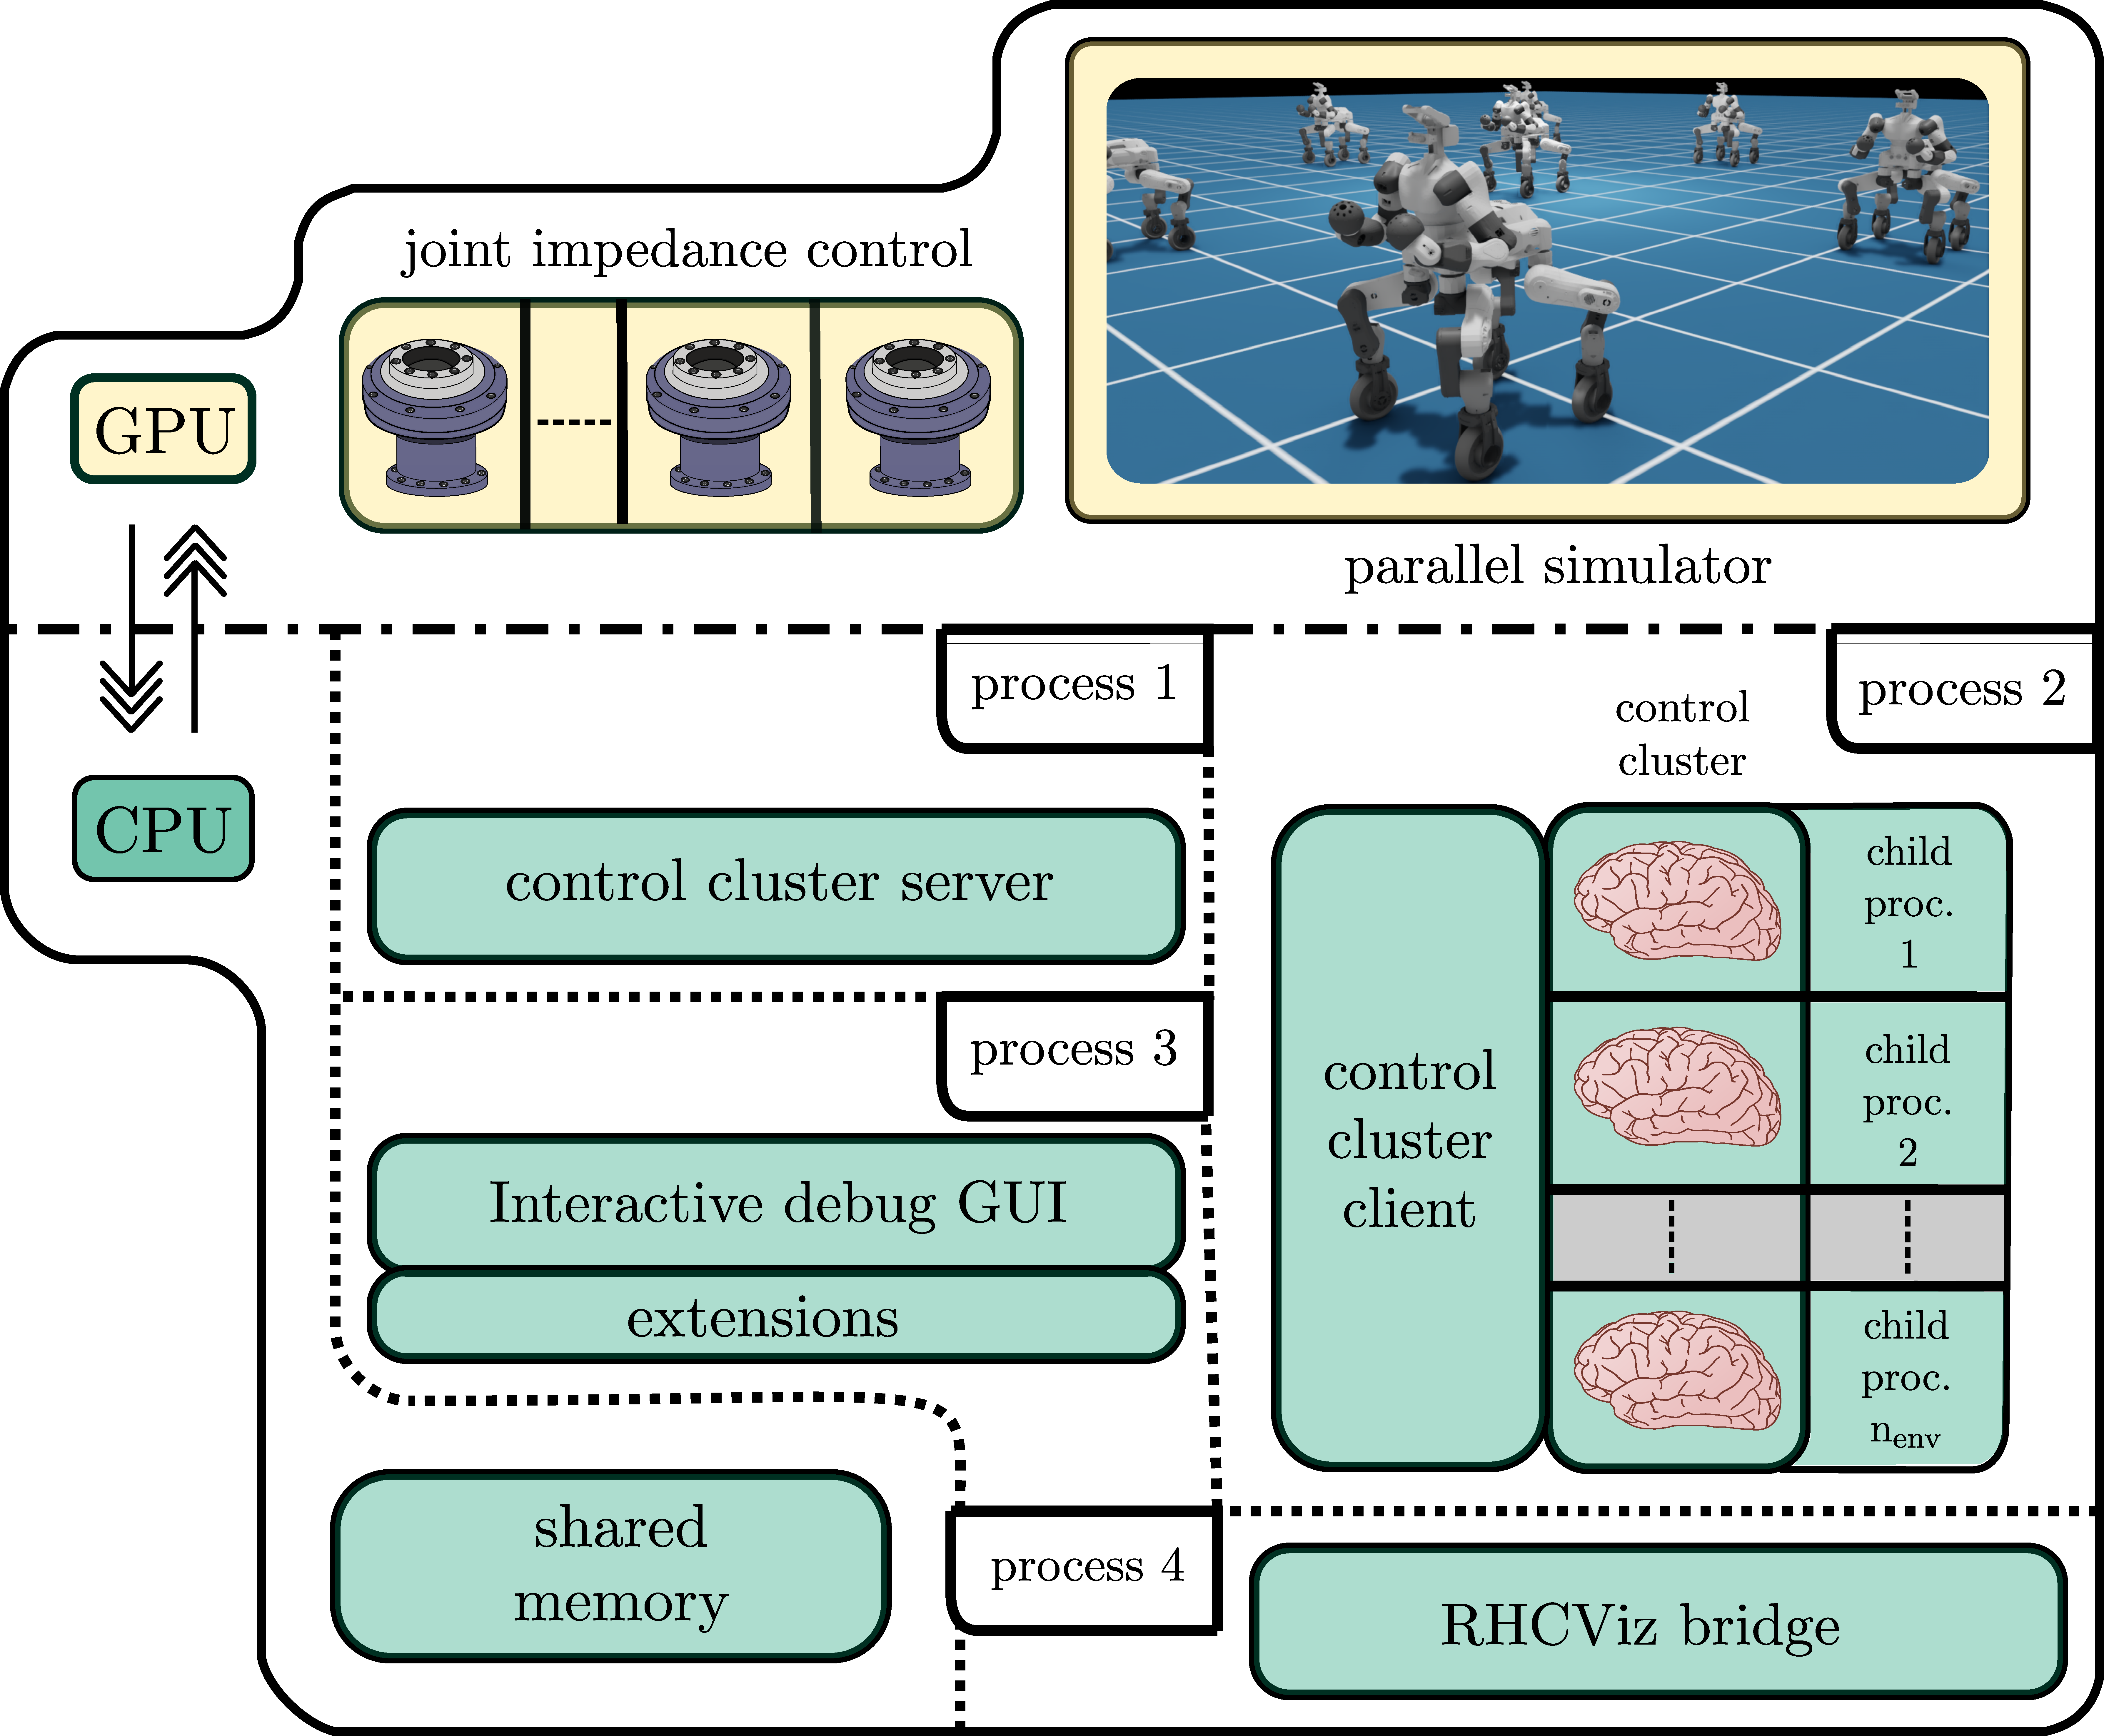
\includegraphics[width=1.0\columnwidth]{imgs/cocluster_arch.pdf}
	\caption{High-level overview of the training environment to which the agent is exposed: the robot in the simulator is controlled through a joint-level impedance controller, which is in turn used by a higher-level receding horizon controller. The agent can indirectly control the robot through the latter.}
	\label{fig:coclbridge_arch}
\end{figure}
\cite{mystuff::lrhccontrol}
\cite{mystuff::omnirobogym}
\cite{mystuff::coclusterbridge}
\cite{mystuff::rhcviz}
\cite{mystuff::sharsoripcpp}

\begin{figure*}[t]
	\centering
	\vspace{0.1cm}
	\includegraphics[width=0.98\textwidth]{imgs/learning_based_rhc.pdf}
	\caption{Our take on Learning-based Receding Horizon Control: a MPC controller is exposed to a RL agent through key runtime parameters, like contact phases, its internal state (costs, constrains..) and interfaces for setting task commands. The agent learns to exploit the underlying RHC controller to perform the tracking of user-specified high-level task references. This allows to both tackle problems which are non-trivial at the MPC level (like phase selection), while also exploiting the flexibility of the agent to complete tasks and the capability of the MPC of ensuring safety.}
	\label{fig:lrhc_arch}
\end{figure*}